%    Copyright (C) 2014 Imperial College London.

%    This file is part of Firedrake-Fluids.
%
%    Firedrake-Fluids is free software: you can redistribute it and/or modify
%    it under the terms of the GNU General Public License as published by
%    the Free Software Foundation, either version 3 of the License, or
%    (at your option) any later version.
%
%    Firedrake-Fluids is distributed in the hope that it will be useful,
%    but WITHOUT ANY WARRANTY; without even the implied warranty of
%    MERCHANTABILITY or FITNESS FOR A PARTICULAR PURPOSE.  See the
%    GNU General Public License for more details.
%
%    You should have received a copy of the GNU General Public License
%    along with Firedrake-Fluids.  If not, see <http://www.gnu.org/licenses/>.

\documentclass[a4paper,11pt]{report}
\usepackage[top=3cm, bottom=3cm, left=3cm, right=3cm]{geometry}
\usepackage{graphicx}
\usepackage{amsmath, amssymb}
\usepackage{hyperref}
\usepackage{natbib}
\bibpunct{(}{)}{;}{a}{,}{,}

\title{Firedrake-Fluids User Manual}
\author{Imperial College London}

\begin{document}

\maketitle
\tableofcontents

\setlength{\parskip}{0.3cm}
\setlength{\parindent}{0cm}

%%%%%%%%%%%%%%%%%%%%%%%%%%%%
%%%%%%% Introduction %%%%%%%
%%%%%%%%%%%%%%%%%%%%%%%%%%%%
\chapter{Introduction}
\section{Overview}
Firedrake-Fluids is a collection of finite element-based numerical models for the study of fluid dynamical systems. It uses the Firedrake framework \citep{ImperialCollegeLondon_2013, Rathgeber_Submitted} to automate the solution of the governing equations written in their weak form using the Unified Form Language (UFL) \citep{Alnaes_etal_2014}.

\section{Automated solution technique}
When a model in Firedrake-Fluids is executed by the Python interpreter, the model's UFL (along with the computational mesh used to discretise the domain) is first passed to the Firedrake framework. Within this framework, the UFL is converted to an abstract syntax tree (AST) by a modified version of the FEniCS Form Compiler (FFC). Additionally, the topology of the mesh is described by a PETSc DMPlex object (\url{http://www.mcs.anl.gov/petsc/petsc-current/docs/manualpages/DM/DMPLEX.html}) to allow the efficient execution of the generated code over the whole mesh.

 This AST is then passed to the PyOP2 library \citep{Rathgeber_etal_2012, Markall_etal_2013} which, after being optimised by the COFFEE compiler and converted into low-level C kernels, targets and compiles the code towards a specific hardware architecture and executes it on that hardware.

As an example, consider the UFL statement in Figure \ref{fig:ufl_expression}. This one single line of UFL is converted to a kernel comprising many lines of C code, which perform the evaluation of the expression, as shown in Figure \ref{fig:c_kernel}.

\begin{figure}
   \centering
   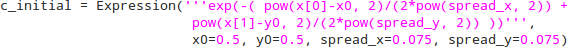
\includegraphics[width=0.75\columnwidth]{images/ufl_expression.png}
   \caption{An example of a UFL expression.}
   \label{fig:ufl_expression}
\end{figure}

\begin{figure}
   \centering
   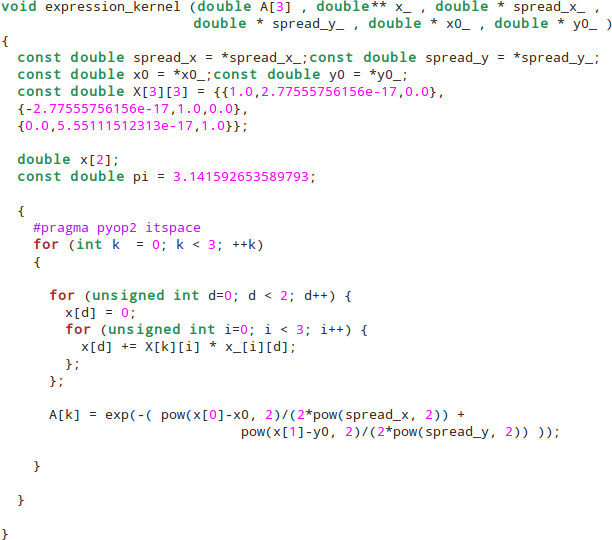
\includegraphics[width=0.75\columnwidth]{images/c_kernel.png}
   \caption{An example of C code, generated automatically, for the purpose of evaluating an expression defined by a high-level, near-mathematical UFL statement.}
   \label{fig:c_kernel}
\end{figure}

\section{Setup}
Before running the models in Firedrake-Fluids, please ensure that all the dependencies specified in the README file are satisfied. Installations for Firedrake (and its dependencies) can be found here: \url{http://www.firedrakeproject.org/download.html}. Firedrake-Fluids also relies on the libspud library (and the Python bindings) to retrieve simulation-related options (e.g. the time-step size and initial conditions) from a configuration/setup file. Following the steps below at the command line will download and build libspud, and install the Python bindings:

\texttt{bzr checkout lp:$\sim$spud/spud/trunk libspud}\\
\texttt{cd libspud}\\
\texttt{./configure}\\
\texttt{make}\\
\texttt{cd python}\\
\texttt{sudo python setup.py install}

Firedrake-Fluids comprises a collection of Python files containing the implementation of the different models; a set of schema files used to define the different options a simulation configuration file can take; and a set of test cases to help ensure the correctness of the models.

%%%%%%%%%%%%%%%%%%%%%%%%%%%%%%%%%%%
%%%%%%% Shallow water model %%%%%%%
%%%%%%%%%%%%%%%%%%%%%%%%%%%%%%%%%%%
\chapter{Shallow water model}
The shallow water model solves the non-linear, non-rotational shallow water equations which describe the dynamics of a free surface and a depth-averaged velocity field. For modelling purposes, the free surface is split up into a mean component $H$ (i.e. the hydrostatic depth to the seabed) and a perturbation component $h$ (see Figure \ref{fig:shallow_water_setup}).

\begin{figure}
   \centering
   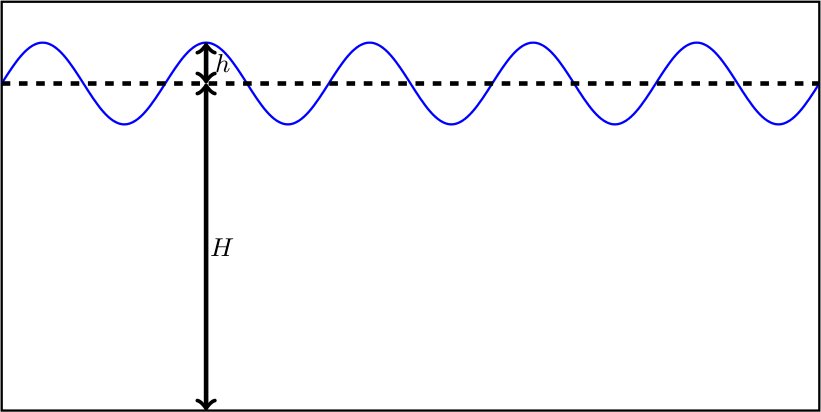
\includegraphics[width=0.6\columnwidth]{images/shallow_water_h_H.png}
   \caption{Single-layer shallow water set-up.}
   \label{fig:shallow_water_setup}
\end{figure}

\section{Model equations}\label{sect:model_equations}
The shallow water equation set comprises a momentum equation and a continuity equation, each of which are defined below. These are defined on a domain $\Omega$ and for a time $t \in [0, T]$.

\subsection{Momentum equation}
The momentum equation is solved in non-conservative form such that
\begin{equation}
   \frac{\partial \mathbf{u}}{\partial t} + \mathbf{u}\cdot\nabla\mathbf{u} = -g\nabla h + \nabla\cdot\mathbb{T} - C_D\frac{||\mathbf{u}||\mathbf{u}}{(H + h)},
\end{equation}
where $g$ is the acceleration due to gravity, $\mathbf{u}$ is the velocity, and $C_D$ is the non-dimensional drag coefficient. The stress tensor $\mathbb{T}$ is given by 
\begin{equation}
   \mathbb{T} = \nu\left(\nabla\mathbf{u} + \nabla\mathbf{u}^{\mathrm{T}}\right) - \frac{2}{3}\nu\left(\nabla\cdot\mathbf{u}\right)\mathbb{I},
\end{equation}
where $\nu$ is the isotropic kinematic viscosity, and $\mathbb{I}$ is the identity tensor.

\subsection{Continuity equation}
The continuity equation is given by
\begin{equation}
   \frac{\partial h}{\partial t} + \nabla\cdot\left(\left(H + h\right)\mathbf{u}\right) = 0.
\end{equation}

\subsection{Discretisation and solving}
The model equations are discretised using a Galerkin finite element method. Essentially, this begins by deriving the weak form of the equations by multiplying through by a test function $\mathbf{w} \in H^1(\Omega)^3$ (where $H^1(\Omega)^3$ is the first Hilbertian Sobolev space \citep{Elman_etal_2005}) and integrating over $\Omega$. In the case of the momentum equation, this becomes
\begin{eqnarray}
   \nonumber\int_{\Omega}\mathbf{w}\cdot\frac{\partial \mathbf{u}}{\partial t}\ \mathrm{dV} + \int_{\Omega}\mathbf{w}\cdot(\mathbf{u}\cdot\nabla\mathbf{u}) \ \mathrm{dV} = -\int_{\Omega}g\mathbf{w}\cdot\nabla h \ \mathrm{dV} + \int_{\Omega}\nabla\mathbf{w}\cdot \mathbb{T} \ \mathrm{dV} \\- \int_{\Omega}C_D\mathbf{w}\cdot\frac{||\mathbf{u}||\mathbf{u}}{(H + h)} \ \mathrm{dV}.
\end{eqnarray}
A solution $\mathbf{u} \in H^1(\Omega)^3$ is sought such that it is valid $\forall \mathbf{w}$.

The solution fields $\mathbf{u}$ and $h$ are each represented by a set of interpolating basis functions, such that
\begin{equation}
   \mathbf{w} = \sum_{i=1}^{N_\mathrm{u\_nodes}} \phi_i\mathbf{w}_i,
\end{equation}
\begin{equation}
   \mathbf{u} = \sum_{i=1}^{N_\mathrm{u\_nodes}} \phi_i\mathbf{u}_i,
\end{equation}
and
\begin{equation}
   h = \sum_{i=1}^{N_\mathrm{h\_nodes}} \psi_ih_i,
\end{equation}
where $\phi_i$ and $\psi_i$ are the basis functions representing the velocity and free surface perturbation fields, respectively; $N_\mathrm{u\_nodes}$ and $N_\mathrm{h\_nodes}$ are the number of velocity and free surface solution nodes, respectively; and the coefficients $\mathbf{u}_i$ and $h_i$ are to be found by a solution method. If the basis functions $\phi_i$ are continuous across each cell/element in the mesh, then the method is known as a \textit{continuous} Galerkin (CG) method, whereas if the basis functions are discontinuous, then the method is known as a \textit{discontinuous} Galerkin (DG) method.

The momentum equation, discretised in space, then becomes a matrix system:
\begin{equation}
   \mathbf{M}\frac{\partial\mathbf{u}}{\partial t} + \mathbf{A}(\mathbf{u})\mathbf{u} + \mathbf{K}\mathbf{u} = -\mathbf{C}h + \mathbf{D}(\mathbf{u}, h)\mathbf{u},
\end{equation}
where $\mathbf{M}$, $\mathbf{A}$, $\mathbf{K}$, $\mathbf{C}$ and $\mathbf{D}$ are the mass, advection, stress, gradient and drag matrices, respectively.

The time-derivative is discretised using the implicit backward Euler method, yielding a fully discrete system of equations:
\begin{eqnarray}
   \mathbf{M}\frac{\mathbf{u}^{n+1} - \mathbf{u}^{n}}{\Delta t} + \mathbf{A}(\mathbf{u}^{n+1})\mathbf{u}^{n+1} + \mathbf{K}\mathbf{u}^{n+1} = -\mathbf{C}h^{n+1} + \mathbf{D}(\mathbf{u}^{n+1}, h^{n+1})\mathbf{u}^{n+1},
\end{eqnarray}
where $\Delta t$ is the time-step.

The finite element method is also applied to the continuity equation, which must be solved along with the momentum equation, yielding a block-coupled system. In Firedrake-Fluids, this system is preconditioned using a fieldsplit preconditioner \citep{Brown_etal_2012} and solved with the GMRES linear solver \citep{SaadSchultz_1986}.

\section{Configuring a simulation}
The configuration/setup of a shallow water simulation in Firedrake-Fluids is defined in a Shallow Water Markup Language (.swml) file. This is essentially an XML file that contains tags/elements which are specific to the context of a shallow water simulation. The full range of possible options that are available to the user are defined by a set of schema files in the \texttt{schemas} directory; these can be thought of as `templates' from which an .swml setup file can be constructed.

Creating a shallow water setup/configuration file is best done using the Diamond graphical user interface (GUI) \citep{Ham_etal_2009} that is supplied with the libspud dependency. At the command line, from the Firedrake-Fluids base directory, creating an .swml file called \texttt{example.swml} can be done using

\texttt{diamond -s schemas/shallow\_water.rng example.swml}

Note that the -s flag is used to specify the location of the schema file \texttt{shallow\_water.rng}, while the final command line argument is the name of the setup file we want to create. The Diamond GUI will look something like the one shown in Figure \ref{fig:diamond}.

\begin{figure}[!ht]
   \centering
   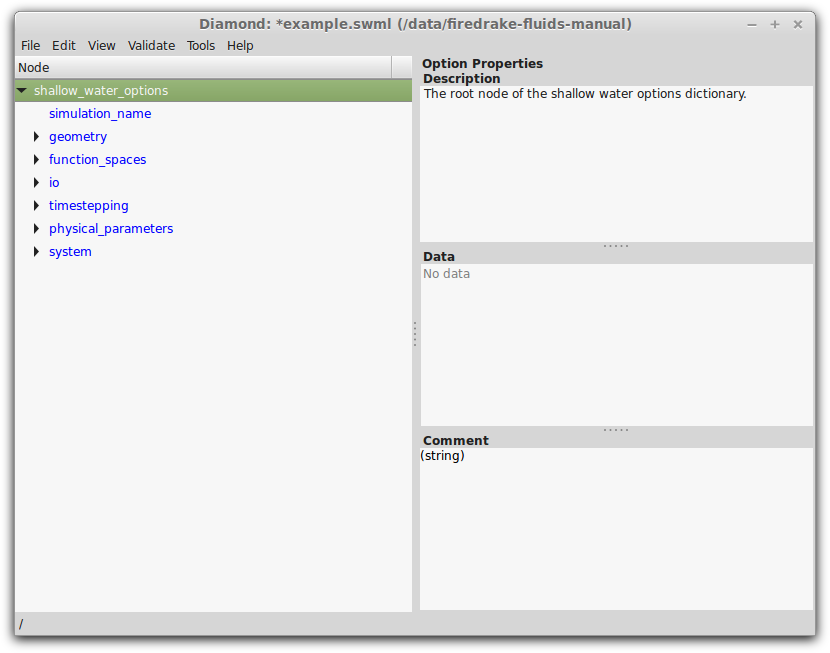
\includegraphics[width=1\columnwidth]{images/diamond.png}
   \caption{The Diamond \citep{Ham_etal_2009} graphical user interface. Notice that all the available options are currently in blue; this means that they still need to be specified the user, after which the font colour will turn black.}
   \label{fig:diamond}
\end{figure}

Details of each of the options (and sub-options underneath, displayed by clicking the black arrows) are given in the following sub-sections.

\subsection{Simulation name}
All simulations must be given a name under \texttt{/simulation\_name}. This name is used when outputting solution files created during the simulation. Please use alpha-numeric characters and avoid using non-standard characters such as ampersands, commas, semi-colons, etc here.

\subsection{Geometry}
The \texttt{/geometry} section of the setup file concerns the dimension of the problem, and the location of the computational mesh used to discretise the domain.

The dimension should be one of the first options to be set. Be careful here; this option can only be set once because other options further down the list rely on it.

In the case of the mesh file location, note that only Gmsh \texttt{.msh} files \citep{GeuzaineRemacle_2009} are supported.

\subsection{Function spaces}
Since two fields, velocity $\mathbf{u}$ and free surface perturbation $h$, have to be solved for in the shallow water model, two function spaces may be specified. In Firedrake-Fluids, the function spaces are assumed to be composed of Lagrange polynomial basis functions. The order of these polynomials can be specified in the \texttt{degree} sub-option of each \texttt{function\_space}. The \texttt{family} refers to whether the basis functions are continuous or discontinous across the cells/elements of the mesh.

\subsection{Input/output (I/O)}
Solution files may be dumped at specific intervals, specified in time units. Setting the \texttt{io/dump\_period} option to zero will result in dumps at every time-step. Note that solution files can currently only be written in VTU format (see \url{http://www.vtk.org} for more information).

Users can also enable checkpointing which allows them to resume the simulation at a later time. The checkpoint data will be written to a file called \texttt{checkpoint.npz}. The time interval between checkpoint dumps can be specified under \texttt{io/checkpoint/dump\_period}. The simulation can be later resumed by specifying the location of this file with the \texttt{-c} flag (see Section \ref{sect:running_a_simulation} for more details).

\subsection{Timestepping}
The time-step $\Delta t$ and finish time $T$ are specified under \texttt{timestepping/timestep} and \texttt{timestepping/finish\_time}, respectively. The \texttt{timestepping/start\_time} (i.e. the initial value of $t$) is usually set to zero.

For simulations which are known to converge to a steady-state, Firedrake-Fluids can stop the simulation when the maximum difference of all solution fields (i.e. $\mathbf{u}$ and $h$) between time $n$ and $n+1$ becomes less than a user-defined tolerance; this is specified in \texttt{timestepping/steady\_state/tolerance}.

\subsection{Physical parameters}
The only physical parameter applicable to the equation set solved in the Firedrake-Fluids shallow water model is the acceleration due to gravity. This is approximately 9.8 ms$^{-2}$ on Earth.

\subsection{System: Core fields}
The model requires three fields to be set up under the \texttt{/system/core\_fields} section of the setup file. These are the key fields used in shallow water simulations, and are named
\begin{itemize}
   \item \textit{Velocity} (a prognostic field, corresponding to $\mathbf{u}$).
   \item \textit{FreeSurfacePerturbation} (a prognostic field, corresponding to $h$)
   \item \textit{FreeSurfaceMean} (a prescribed field, corresponding to $H$)
\end{itemize}
It is here that the initial and boundary conditions for the fields can be specified. These can either be constant values, or values defined by a C++ expression.

\subsubsection{C++ expressions}
Non-constant values for initial and boundary conditions can be specified under the \texttt{cpp} sub-option; here, a Python function needs to be written which returns a string containing a C++ expression. An example is given in Figure \ref{fig:cpp_expression}.

\begin{figure}[!ht]
   \centering
   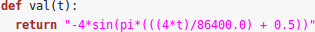
\includegraphics[width=0.5\columnwidth]{images/cpp_expression.png}
   \caption{An example of a Python function returning a string containing a C++ expression. This C++ expression is used to define the non-constant values of a boundary condition. The function must be called \texttt{val} and have the argument \texttt{t}, which is the current simulation time that may be included in the C++ expression. The variable \texttt{x} contains the coordinates of the domain (i.e. \texttt{x[0]}, \texttt{x[1]} and \texttt{x[2]} are the $x$, $y$, and $z$ coordinates, respectively).}
   \label{fig:cpp_expression}
\end{figure}

\subsubsection{Boundary conditions}
A new boundary condition can be created for a given field by clicking the \texttt{+} button next to the gray \texttt{boundary\_condition} option. Each boundary condition must be given a unique name.

The surfaces on which the boundary conditions need to be applied should be specified under \texttt{boundary\_condition/surface\_ids}; multiple surface IDs should be separated by a single space. The type of boundary condition should then be specified along with its value; the available types are (for velocity):
\begin{itemize}
   \item \textit{Dirichlet}: Strong Dirichlet boundary conditions can be enforced for both the FreeSurfacePerturbation and Velocity fields by selecting the \texttt{dirichlet} type.
   \item \textit{No-normal flow}: Imposing a no-normal flow condition for velocity (i.e. $\mathbf{u}\cdot\mathbf{n} = 0$) can currently only be done weakly by integrating the continuity equation by parts (by enabling the \texttt{/system/equations/continuity\_equation/integrate\_by\_parts} option) and selecting the \texttt{no\_normal\_flow} boundary condition type.
   \item \textit{Flather}: A \cite{Flather_1976} open boundary condition can be imposed weakly by integrating the continuity equation by parts and selecting the \texttt{flather} boundary condition type in the configuration options. This boundary condition enforces:
   \begin{equation}
      \mathbf{u} = \mathbf{u}_{\mathrm{exterior}} - \sqrt{\frac{g}{H}}\left(h - h_{\mathrm{exterior}}\right),
   \end{equation}
   where $\mathbf{u}_{\mathrm{exterior}}$ and $h_{\mathrm{exterior}}$ are the known/expected values for velocity and the free surface perturbation. Any difference between the exterior values and the simulated values along the boundary is allowed out of the domain in such a way that minimises spurious reflections.
\end{itemize}

For the free surface perturbation field $h$, only Dirichlet boundary conditions are available.

\subsection{System: Equations}
As already described in Section \ref{sect:model_equations}, there are two equations which make up the shallow water model: the momentum equation and the continuity equation. Options for both of these fields, concerning their discretisation and parameters (e.g. for $C_D$ and $\nu$), can be found under \texttt{/system/equations/momentum\_equation} and \texttt{/system/equations/continuity\_equation}.

\subsubsection{Spatial discretisation}
The spatial discretisation (continuous or discontinuous Galerkin) currently depends on the continuity of the function spaces in use, rather than on the choices made in this option. However, if \texttt{continuous\_galerkin} is selected, there are stabilisation-related sub-options available to stabilise the advection term when using CG. See Chapter \ref{chap:stabilisation} for more information on the stabilisation schemes available.

\subsubsection{Mass term}
An option is available to exclude the mass term in the momentum (or continuity) equation, under \texttt{../mass\_term/exclude\_mass\_term}.

\subsubsection{Advection term}
An option is available to exclude the advection term in the momentum (or continuity) equation, under \texttt{../advection\_term/exclude\_advection\_term}. The advection term may also be integrated by parts by enabling the \texttt{../advection\_term/integrate\_by\_parts} option; this is required for the imposition of weak velocity boundary conditions.

\subsubsection{Drag term}
To include the quadratic drag term in the momentum equation, the \texttt{drag\_term} option must be enabled under \texttt{/system/equations/momentum\_equation/} and the non-dimensional drag coefficient $C_D$ should be specified.

\subsubsection{Stress term}
To include the stress term in the momentum equation, the \texttt{stress\_term} option must be enabled and the isotropic, kinematic physical viscosity of the fluid $\nu$ must be specified.

\subsubsection{Turbulence parameterisation}
By default, the momentum equation does not account for turbulent Reynolds stresses. However, if the \texttt{turbulence\_parameterisation} option is enabled, then the Reynolds stresses can be parameterised through the calculation of an eddy viscosity, which models the effects of small-scale eddies on the large-scale flow turbulence. This eddy viscosity is added to the background viscosity $\nu$ in the stress term. More information can be found in Chapter \ref{chap:turbulence_parameterisation}.

\subsubsection{Source term}
An additional user-defined source term can be added to the right-hand side of the equation under consideration via the \texttt{source\_term} sub-option.

\section{Running a simulation}\label{sect:running_a_simulation}
A shallow water simulation can be run by executing the \texttt{shallow\_water.py} file with the Python interpreter, and providing the path to the .swml simulation configuration file. An example would be:

\texttt{python models/shallow\_water.py example.swml}

from the Firedrake-Fluids base directory. Available flags for the shallow water model are:

\begin{itemize}
   \item \texttt{-c}: Initialise a simulation from a specified checkpoint file.
   \item \texttt{-h}: Display a help message.
\end{itemize}

\section{Current limitations}
\begin{itemize}
   \item When using a discontinuous Galerkin method, the form of the stress tensor is currently restricted to:
   \begin{equation}
      \mathbb{T} = \nu\nabla\mathbf{u}.
   \end{equation}
   \item When using a discontinuous Galerkin discretisation, the interior penalty method \citep{Arnold_etal_2002} is the only method available for determining the value of $\nabla\mathbf{u}$ at the discontinuous interior element boundaries. Similarly, only a simple upwinding method can be used to determine $\mathbf{u}$ along interior element boundaries.
\end{itemize}


%%%%%%%%%%%%%%%%%%%%%%%%%%%%%%%%%%%%%
%%%%%%% Stabilisation methods %%%%%%%
%%%%%%%%%%%%%%%%%%%%%%%%%%%%%%%%%%%%%
\chapter{Stabilisation methods}\label{chap:stabilisation}
When using a continuous Galerkin discretisation in advection-dominated problems, it may be necessary to stabilise the advection term in the momentum equation.

The implementation of the stabilisation methods can be found in the file \texttt{stabilisation.py}.

\section{Streamline upwind}


%%%%%%%%%%%%%%%%%%%%%%%%%%%%%%%%%%%%%%%%%%%
%%%%%%% Turbulence parameterisation %%%%%%%
%%%%%%%%%%%%%%%%%%%%%%%%%%%%%%%%%%%%%%%%%%%
\chapter{Turbulence parameterisation}\label{chap:turbulence_parameterisation}
This chapter describes the turbulence models that are available in Firedrake-Fluids.

\section{Large Eddy Simulation (LES)}
The UFL implementation of all LES models can be found in the file \texttt{models/les.py}.

\subsection{Smagorinsky model}
The \cite{Smagorinsky_1963} model calculates an eddy viscosity $\nu^\prime$
\begin{equation}
   \nu^\prime = \left(C_s\Delta_e\right)^2|\mathbb{S}|,
\end{equation}
where $C_s$ is the Smagorinsky coefficient which is typically between 0.1 and 0.2 \citep{Deardorff_1971}, and $\Delta_e$ is some measure of the element size. Here it is given by the square root of the element's area in 2D, or cube root of the element's volume in 3D. The term $|\mathbb{S}|$ is the modulus of the strain rate tensor $\mathbb{S}$:
\begin{equation}
 \mathbb{S} = \frac{1}{2}\left(\nabla\mathbf{u} + \nabla\mathbf{u}^{\mathrm{T}}\right).
\end{equation}
The eddy viscosity $\nu^\prime$ is added to the background/physical viscosity of the fluid, thereby contributing to the stress term in the momentum equation.

%%%%%%%%%%%%%%%%%%%%%%%%%%%%%%%%%
%%%%%%% Diagnostic fields %%%%%%%
%%%%%%%%%%%%%%%%%%%%%%%%%%%%%%%%%
\chapter{Diagnostic fields}
Some stand-alone functions are available in the \texttt{diagnostics.py} file for computing flow diagnostics.

\section{Courant number}
The Courant number diagnostic computes the field defined by
\begin{equation}
   \frac{||\mathbf{u}||\Delta t}{\Delta x},
\end{equation}
where $\Delta t$ is the time-step size and $\Delta x$ is the element size (more specifically, it is twice the element's circumradius).

\section{Divergence}
This diagnostic field computes the divergence
\begin{equation}
   \nabla\cdot\mathbf{u},
\end{equation}
of a vector field $\mathbf{u}$.

\bibliographystyle{plainnat}
\bibliography{manual}

\end{document}
